\chapter{Leggibilità}
\begin{mdframed}[style=mystyle,frametitle=]
       La tipografia è come la musica! non sono le note che fanno una melodia, ma è come queste vengono ritmate.
       Lo stesso è la tipografia, dove le note sono i caratteri e il ritmo è dettato da spazi bianchi e neri
    \end{mdframed}
\section{Leggibilità vs Visibilità}
la \hl{leggibilità} riguarda il \textbf{\textit{comfort/facilità con cui l'occhio riesce a scansionare i caratteri}} e azionare il meccanismo mentale che collega testo a significato, senza interruzioni 
\\\\
la \hl{visibilità}, invece, è una variabile che \textbf{\textit{ha a che fare con componenti fisiche, ambientali}}, dello spazio... (es. lo spazio tra occhio e testo, presenza di barriere/intralci)
\\\\
i due si influenzano l'un l'altro ma è bene tenere a mente la distinzione

    \begin{mdframed}[style=mystyle,frametitle=Paradosso dei caratteri gotici]
       negli anni 50, in Germania, sono tornati di moda i caratteri gotici,  categorizzati però come caratteri visibili ma non leggibili. Questo, però, è dovuto al fatto che l'"occhio contemporaneo" non è abituato a questo tipo di carattere, e ciò causa una frequente interruzione in fase di scansione dovuta ai tratti verticali molto spessi, in forte contrasto con le altre linee
    \end{mdframed}

\section{Forma dei caratteri}
Si è analizzato e studiato che la forma del carattere, il suo bilanciamento, influisce sulla leggibilità in maniera significativa.
\\\\
è stato provato che, caratteri con grazie ed in generale caratterizzati dall'armonia e precisione delle monumentali romane, sono tipologie di caratteri che facilitano e rendono fluida la scansione e la lettura. Sono quindi caratteri con \hl{alta leggibilità}
\\\\
La scelta del carattere, quindi, è basata sullo scopo e sulla leggibilità che si deve ottenere
\begin{figure}[H]
    \centering
    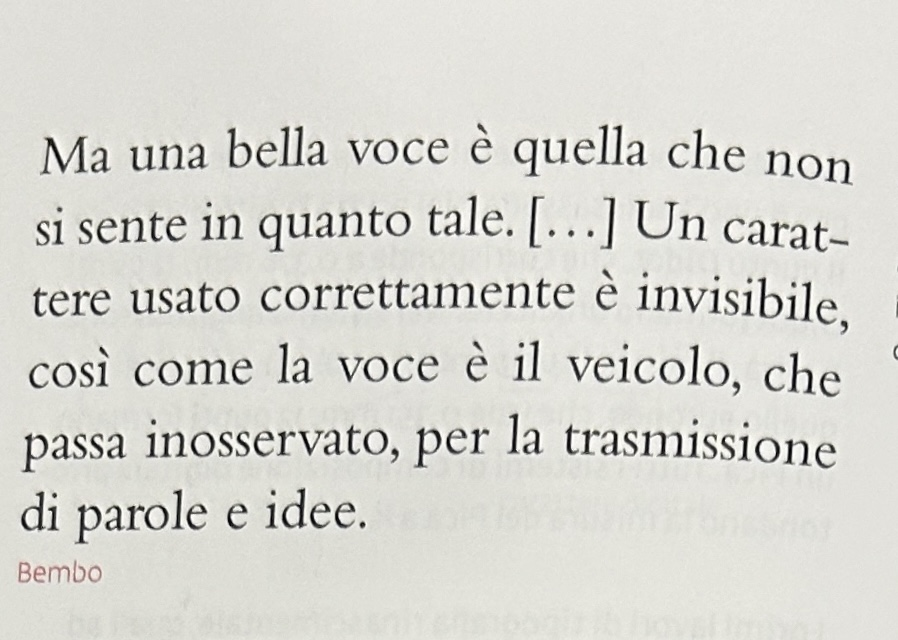
\includegraphics[width=0.2\linewidth]{lzione_4/imgs/f.jpg}
     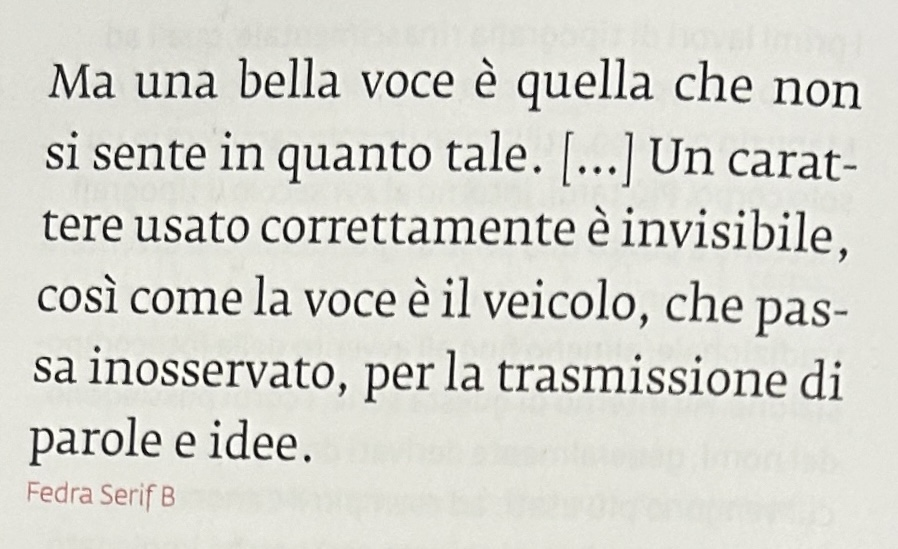
\includegraphics[width=0.2\linewidth]{lzione_4/imgs/f2.jpg}
      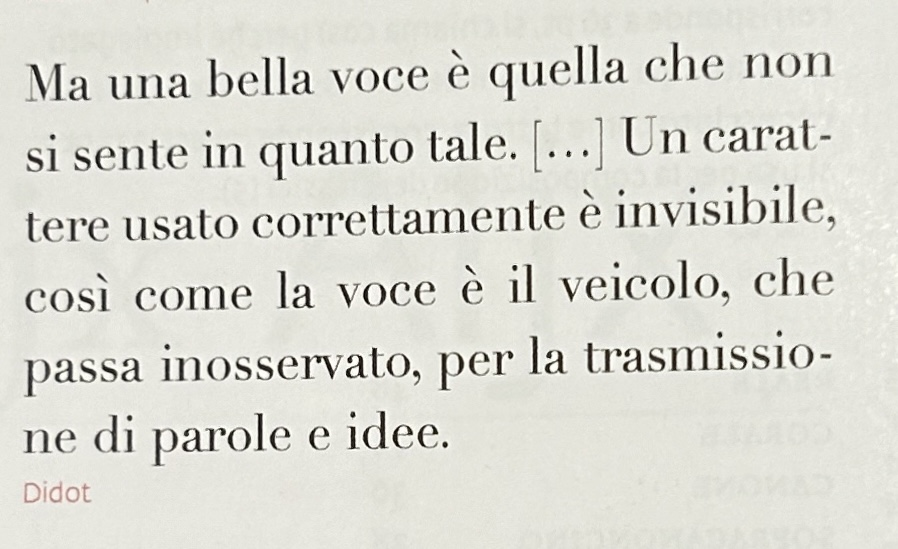
\includegraphics[width=0.2\linewidth]{lzione_4/imgs/f3.jpg} 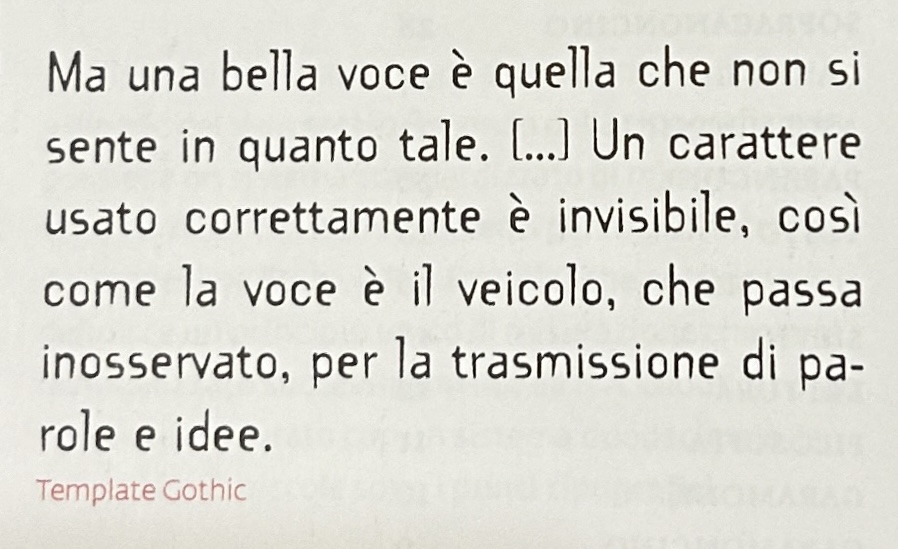
\includegraphics[width=0.2\linewidth]{lzione_4/imgs/f4.jpg}
\end{figure}
Come si può notare, i primi 2 testi, avendo grazie e un ottimo bilanciamento (\hl{poco contrasto tra linee verticali e orizzontali/curve}) tra le forme, risultano nettamente più leggibili rispetto agli altri 2

\subsection{Forma delle minuscole}
La forma di base con cui sono progettate le lettere minuscole influiscono sulla leggibilità.
\\\\
Soprattutto \hl{ la parte alta della lettera minuscola}, infatti, ci permette di identificare uno specifico carattere minuscolo rispetto ad un altro.
Questo fa si che, nel momento della scansione visiva da sx a dx, viene fatta anche una scansione da alto a basso, permettendoci quindi di recepire la lettera più rapidamente
\begin{figure}[H]
    \centering
    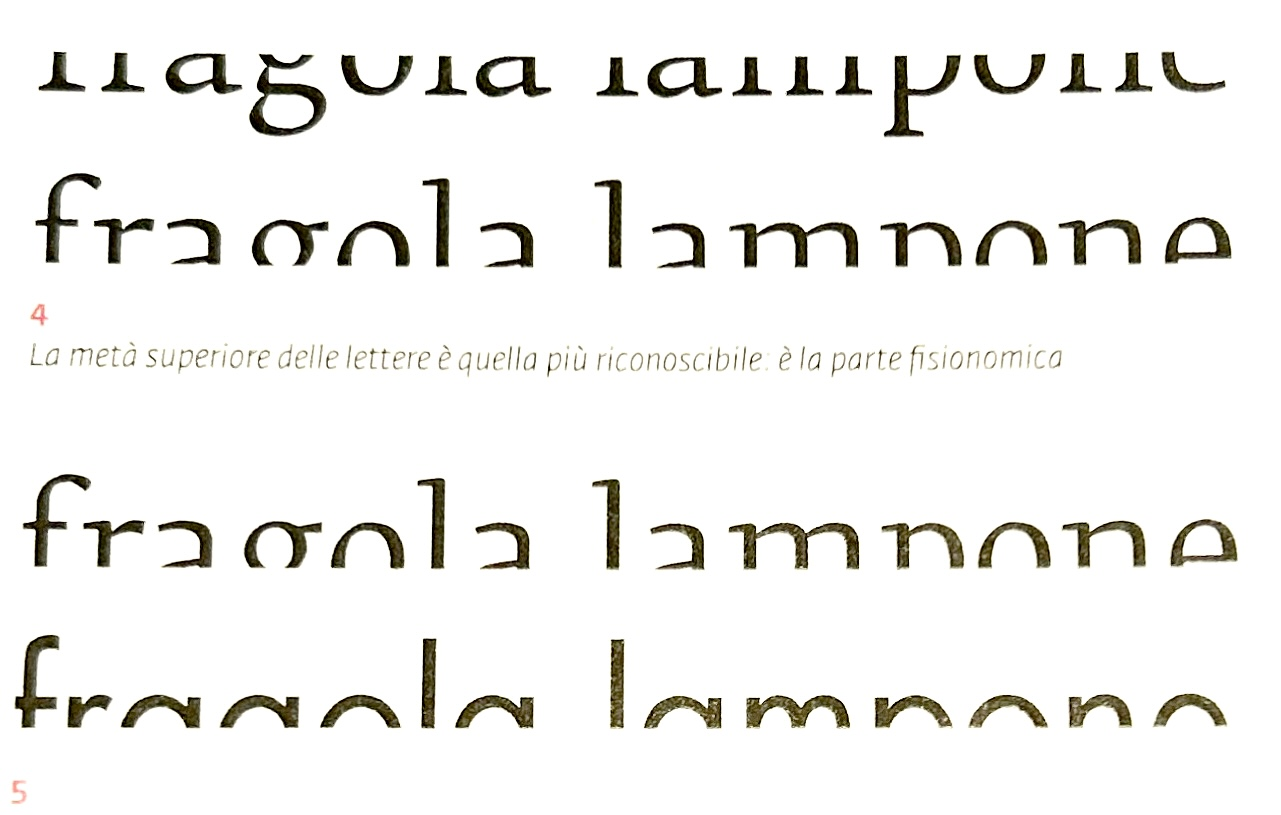
\includegraphics[width=0.3\linewidth]{lzione_4/imgs/f5.jpg}
\end{figure}
\subsection{Approfondimento: come l'occhio e il cervello scansionano le parole}
Il meccanismo alla base della comprensione delle parole in fase di lettura è molto complesso, ma può essere semplificato dicendo che \hl{il nostro cervello non opera scansionando ogni singola lettera di una parola, per poi raggrupparle e associarci un significato}, bensì \hl{percepisce direttamente la forma della parola}; infatti, in nostro cervello conosce perfettamente le forme delle lettere e, rapidamente, riesce a crearne una forma
\\\\
Questo vale soprattutto per le lettere minuscole, che \hl{hano maggior varietà di forme} rispetto alle maiuscole
\begin{figure}[H]
    \centering
    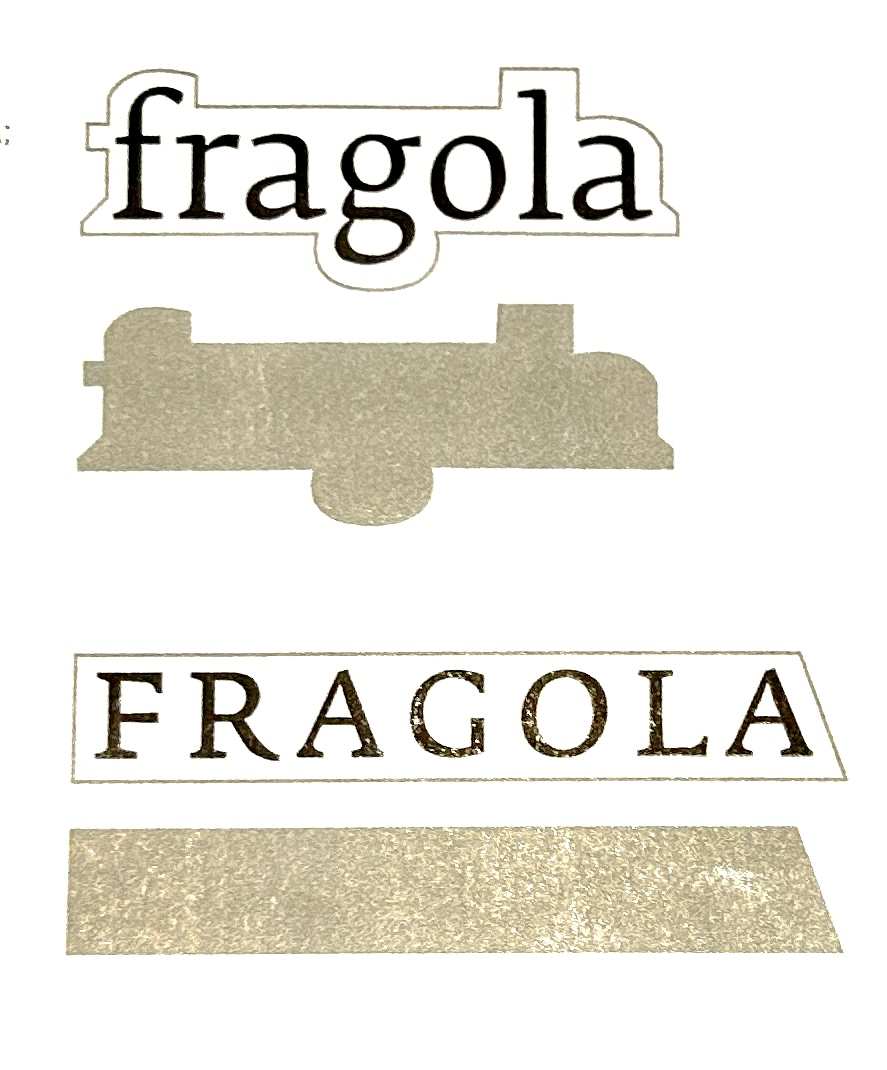
\includegraphics[width=0.3\linewidth]{lzione_4/imgs/f6.jpg}
\end{figure}
 \section{Spaziatura}
La spaziatura è un parametro che influisce moltissimo sulla leggibilità. 
    
\\\\Quando si parla di spaziatura, ci sono diverse tipologie: crenatura, avvicinamento, spaziatura automatica e ottica
\\\\
L'immagine di seguito ci da l'idea di cosa significhi una buona e una brutta spaziatura: nella colonna di sx si nota come, applicando la medesima spaziatura fra le lettere (avvicinamento), si ottiene un risultato otticamente sbagliato

Nella seconda, invece, la spaziatura rende otticamente corretta la parola (crenatura corretta)
\begin{figure}[H]
    \centering
    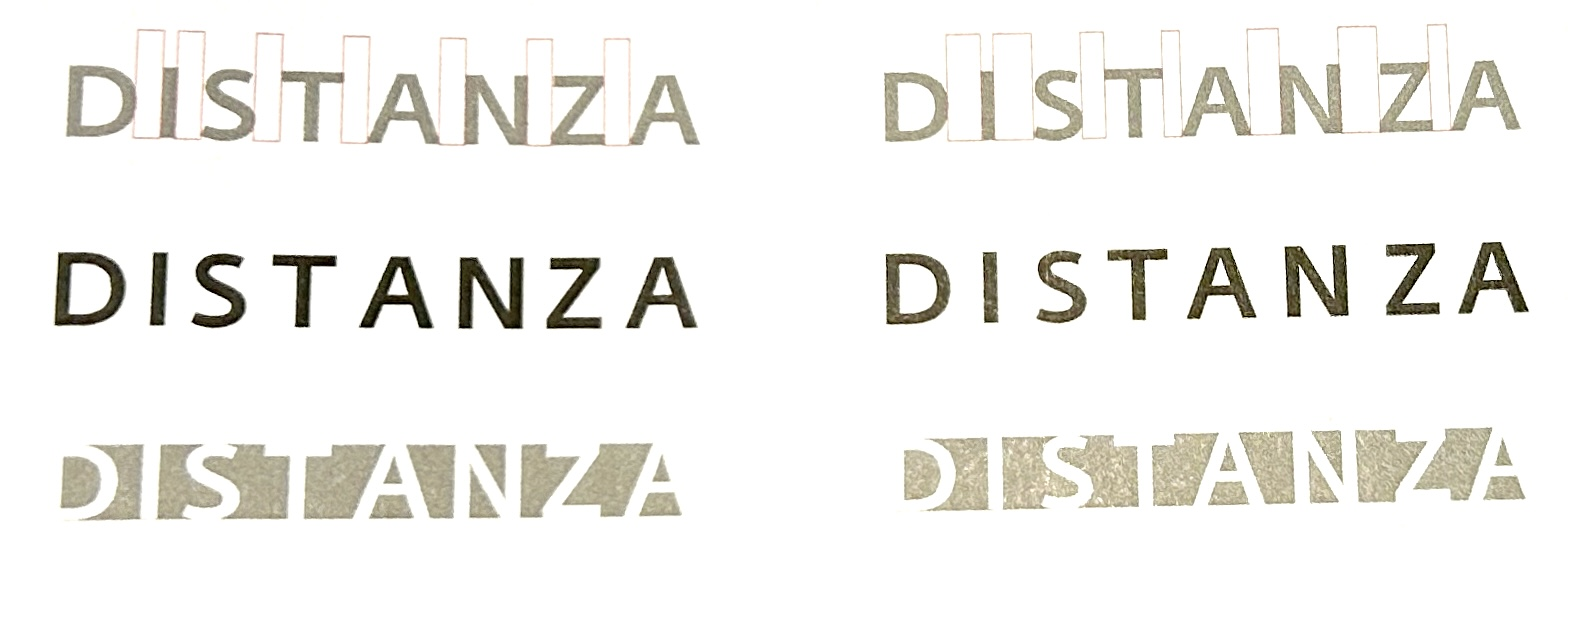
\includegraphics[width=0.2\linewidth]{lzione_4/imgs/f7.jpg}
\end{figure}
    \subsection{Crenatura vs Avvicinamento}
    \subsubsection{Crenatura o Kerning}
    Spaziatura tra \hl{coppie} di lettere, \hl{sulla base della specifica combinazione dei 2 caratteri} in modo tale che il secondo sia in armonia con il precedente 
    \subsubsection{Avvicinamento o Tracking}
    Spaziatura \hl{regolare/costante tra caratteri} in un contesto di più parole. Spesso il tracking è usato per creare una sorta di \hl{gerarchia tra parole}

    \begin{mdframed}[style=mystyle,frametitle=Tip]
        L'avvicinamento è tendenzialmente usato \hl{esclusivamente sui caratteri maiuscoli}, in quanto, con le minuscole, l'effetto ottenuto è tendenzialmente meno apprezzabile rispetto alla medesima parola in maiuscolo.
        \\\\
        Questo è dovuto al fatto che le lettere minuscole derivano dalla scrittura a mano e veloce, quindi questo aumento di spazio così evidente risulta innaturale
    \end{mdframed}

    \subsection{Spaziatura automatica vs Spaziatura ottica}
    in fase di progettazione di un carattere il type dsigner progetta ogni singola e possibile combinazione tra caratteri, in modo tale che l'utilizzatore, poi, possa usare quei caratteri senza badare troppo alla spaziatura corretta.
    
    
    \subsubsection{Spaziatura automatica}
    Quando si ha a ce fare con un testo lungo, quindi, è possibile (sui software) sfruttare la \hl{spaziatura automatica} fra i caratteri, ossia quella progettata dal type designer.
    Questo perchè, in linea di massima, questa spaziatura \hl{è pensata per essere funzionale con testi}
     \subsubsection{Spaziatura ottica}
     specialmente nel caso in cui abbiamo a che fare con titoli/loghi grandi, è consigliabile applicare la \hl{spaziatura ottica}per agevolare ancora di più la resa delle parole, e soprattutto \hl{far notare meno eventuali sbilanciamenti non percepibili in caso di testi lunghi}. Questo perchè in queste casistiche l'occhio si deve concentrare su una singola o poche parole, notando quindi più facilmente possibili problematiche


    \subsection{Spazio vs Distanza}
    Spesso di tende a utilizzare questi 2 termini come sinonimi ma, in realtà, sono due concetti ben diversi!
        \subsubsection{Spazio}
        è l'\hl{area compresa tra 2 caratteri}
        \subsubsection{Distanza}
        è la \hl{"misura" compresa tra 2 caratteri }, ossia la misura tra il punto più a dx di un carattere e quello più a sx dell'altro 
    \begin{figure}[H]
        \centering
        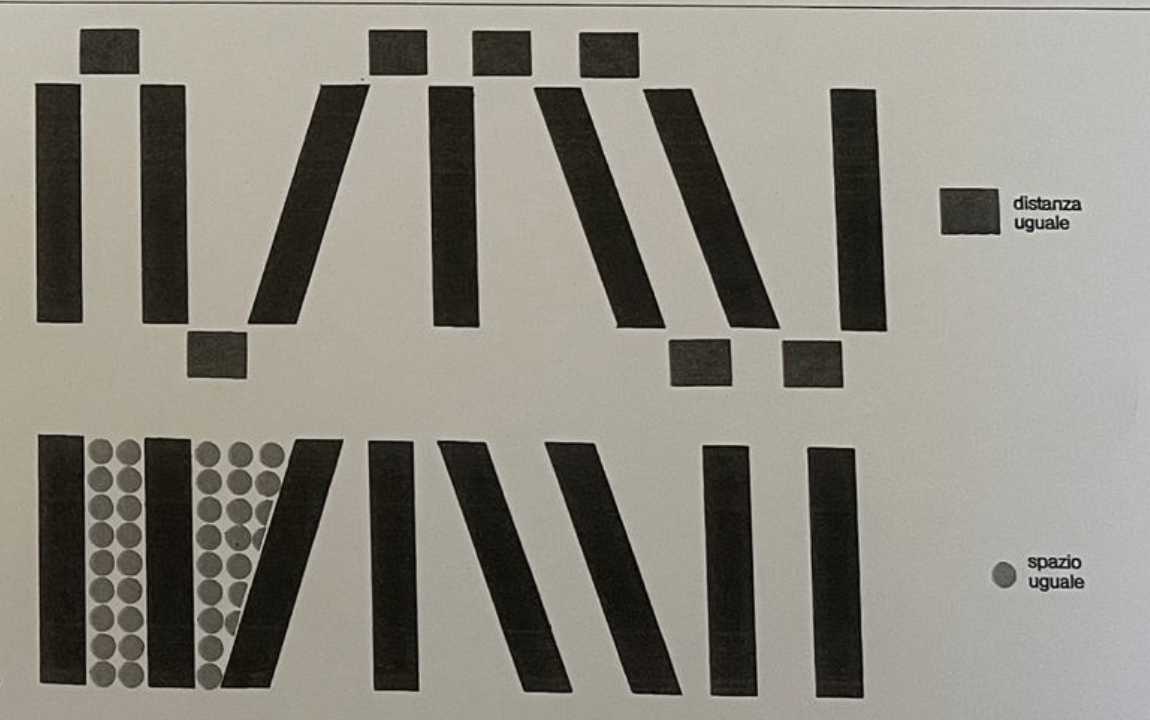
\includegraphics[width=0.2\linewidth]{lzione_4/imgs/Screenshot 2024-11-20 alle 23.42.15.png}
    \end{figure}

\subsection{Il "grigio uniforme"}
a livello teorico, la scrittura utilizzando la corretta spaziatura tra caratteri e parole dovrebbe portare a una percezione, in fase di lettura, di zone a \hl{grigio uniforme}, ossia \hl{il corretto bilanciamento tra spazia bianchi e neri} porta ad avere questa percezione.
\\\\
C'è chi dice inoltre che la tipografia non si basa sul rapportare l'inchiostro nero allo sfondo, bensì il contrario: \hl{la tipografia è in realtà l'uso dello sfondo bianco che, attraverso sei segni di inchiostro, ci da la percezione delle parole}.

Il lavoro del tipografo è quindi quello di trovare il giusto \hl{RITMO} tra spazi bianchi e neri

\subsection{Da dove deriva l'idea di spazio tra caratteri}
il concetto di gestione della spaziatura deriva dalla \hl{stampa tradizionale}, dove ogni lettera era incisa su un punzone (prima in legno, piombo, acciaio e ora esclusivamente digitale).

Un punzone non era niente altro che un blocchetto realizzato a mano inciso. Il problema era però che \hl{i blocchetti non potevano essere sovrapposti per ottenere spaziature piccole}. Di conseguenza si è pensato di creare parti "a sbalzo" del blocchetto per poter avvicinare nel modo giusto i caratteri in base a quello che lo precedeva.

Ne deriva che era necessario avere, per ogni carattere, un set di blocchetti diversi per potersi adattare agli accostamenti con caratteri.

Da qui nasce l'idea della crenatura

        